\section{Preliminaries}
\paragraph{Notations and definitions}
Let $[n] = \{1,\ldots,n\}$, %A 0-1 cube is $\{0,1\}^n$, and a norm-1 cube is $\{-1,1\}^n$ for some integer $n >0$. 
$\R_+ = [0,\infty)$ and $\Z_+$ be the set of positive integers. For a matrix $M\in \R^{m\times n}$, $M^T$ denotes its transpose. For any vector $v\in \R^n$, $\ACTL(v)$ is an $n\times n$ diagonal matrix, with diagonal values $v$. Let $e_n = (1,\ldots, 1)\in \R^n$ be an $n$-dimensional vector of all $1$'s, and $I = \ACTL(e_n)$ is the identity matrix. 
%For any vector $v=(v_1,\ldots,v_n)\in \R^n$, $\ACTL(v)$ is an $n\times n$ diagonal matrix, with diagonal values $v$. Let $e_n = (1,\ldots, 1)\in \R^n$ be an $n$-dimensional vector of all $1$'s; and $I_n = \ACTL(e_n)$, the identity matrix. 
%If $u, v\in \R^n$, let $\inprod{u,v}$ be the inner product of $u$ and $v$: $\inprod{u,v} = \sum_{i=1}^n u_iv_i$.
Let $\norm{v}_p$ denote the $\ell_p$ norm of $v$: 
\[\norm{v}_p = \sqrt[\leftroot{-1}\uproot{8}\scriptstyle p]{\sum_{i=1}^n |v_i|^p}.\]
The canonical Euclidean norm is then $\norm{v}_2$, and another commonly considered attack on the input is the $\ell_\infty$-attack:
\[
\norm{v}_\infty = \max_{i\in[n]}{|v_i|}.
\]
%We use $q$ to denote the Hölder conjugate of $p$ as a convention, i.e., $\frac{1}{p} + \frac{1}{q}=1$. If $v$ is an operator in the $\ell_p$-space, the operator norm of $v$ is then $\norm{v}_q$. 
Throughout the paper, we consider the $\ell_p$-norm of the input's perturbation for $p\geq 1$.
%, and therefore, the $\ell_q$-norm of the gradient, which acts as an operator on the perturbation.

For a matrix $N$, $\eig(N)$ denotes the eigenvalues of $N$. An $n\times n$ symmetric matrix $M\succeq 0$ means that $M$ is positive semidefinite (PSD). There are three common equivalent conditions for $M\succeq 0$:
\begin{enumerate}
\item All eigenvalues of $M$ are non-negative, i.e., $\eig_{\min}(M)\geq 0$;
\item $x^T M x \geq 0$ for all $x\in \R^n$;
\item $\exists L\in \R^{n\times m}$ such that $ LL^T = M$, where $m\in \Z_+$.
\end{enumerate}
Let $\trace(M)$ be the trace of a square matrix $M$: $\trace(M)=\sum_{i=1}^n M_{ii}.$
The Frobenius inner product of two matrices $A\in \R^{m\times n}$ and $B\in \R^{m\times n}$ is 
\[\inprod{A, B}_F = \trace{(A^TB)}=\sum_{i=1}^m\sum_{j=1}^nA_{ij}B_{ij}.\] A vector function $f: \R^n\rightarrow \R^m$ is an affine transformation if $f(x) = Wx + b$ for $W\in \R^{m\times n}$ and $b\in \R^m$. For two functions $f$ and $g$, $f\func g(x) = f(g(x))$ denotes the composition of $f$ and $g$.

Given two metric spaces $(X, d_X)$ and $(Y, d_Y)$, a function $f: X\rightarrow Y$ is \emph{Lipschitz} continuous if there exists $K > 0$ such that for all $x_1, x_2\in X$,
\begin{equation}\label{eq:lipDef}
    d_Y(f(x_2), f(x_1))\leq Kd_X(x_2, x_1).
\end{equation}
The smallest such $K$ satisfying~\cref{eq:lipDef}, denoted by $K_f$, is called the Lipschitz constant of $f$.

\paragraph{Feed-forward networks}
We start with the standard feed-forward structures.  A neural network $f:\R^m\rightarrow \R^l$ is a composition of affine transformations and activation functions:
\[
f_1(x)=  W^{(1)} x+b^{(1)};\; f_i(x)=  W^{(i)}\act(x)+b^{(i)}, i=2,\ldots,d.
\]
where $W^{(i)}\in \R^{n_{i+1}\times n_{i}}$ is the weight matrix between the layers, $n_1 = m$ and $n_{d+1}=l$, $d$ is the depth of the network, and $b^{(i)}\in \R^{n_{i+1}}$ is the bias term. $\act$, the activation, is an element-wise non-linear function. $f = f_d\func\cdots\func f_1$. 

$f: \R^m\rightarrow \R^l$ has $l$ outputs. Let $f^{(i)}$ be the $i$-th output of $f$. The classification of an input $x$ is $\class(f,x)=\argmax_{i\in[l]}f^{(i)}(x)$. Suppose that the prediction of $x$ is $j$, then $f^{(j)}(x)> f^{(k)}(x)$ for all $k\neq j$. The output of $f$ is called the logit score, and the classification model outputs the class with the highest logit score.

$\Tilde{x}$ is an \emph{adversarial attack} for $x$ if $\norm{\bar{x}-x}_p\leq \epsilon$ and $\class(f,\Tilde{x}) \neq j$.

We use $z$ to denote the output of the $(d-1)$-th layer, the representation layer of the network. Let $w^{(i)}_j$ be the $j$-th row of $W^{(i)}$, then $f^{(i)}(x) = w_j^{(d)}z+b^{(d)}_j$. Verifying whether a prediction changes amounts to maximizing $(w^{(d)}_kz+b^{(d)}_k)-(w^{(d)}_jz+b^{(d)}_j) = (w^{(d)}_k-w^{(d)}_j)z+(b^{(d)}_k-b^{(d)}_j)$. If the maximum value is negative for all $k\neq j$, then this prediction is robust. Therefore, we can use a vector $v$ to denote $w^{(d)}_k-w^{(d)}_j$ and a scalar $c$ to denote $b^{(d)}_k-b^{(d)}_j$. From now on, let us assume $l=1$.

In this paper, we focus on the $\relu$ activation function~\cite{relu}, due to its broad applicability, and the verification literatures often study it~\cite{Baader2020Universal,reluplex,chen2020semialgebraic}. $\relu(x) = \max(x, 0)$ is a piece-wise linear function. \Cref{fig:relu} shows the definition of $\relu$ and its plot. In~\cref{sec:other-act}, we discuss other activation functions than $\relu$. 
    \begin{figure}\normalsize
    
    %\textbf{
    %    Intepretation}
    %\vspace{1em}

    %\begin{subfigure}%{.3\textwidth}
        \centering
        %\begin{scaletikzpicturetowidth}{\textwidth}
        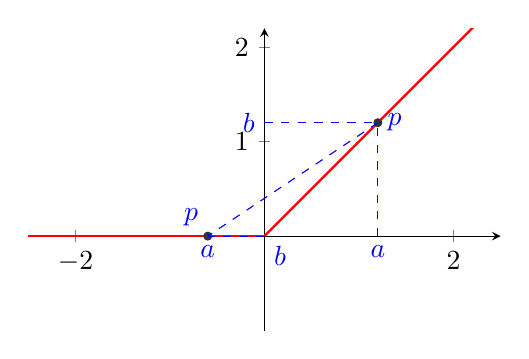
\begin{tikzpicture}
            \begin{axis}[
                axis lines=middle,
                y=1.2cm,
                x=1.2cm,
                xmax=2.5,
                xmin=-2.5,
                xtick={-2,0, 2},
                ymin=-1,
                ymax=2.2,
                ytick={0,1, 2},
                width=2cm
            ]
        
        
            \addplot [domain=-10:0, samples=100,
                      thick, red] {0};
                
            \addplot [domain=0:10, samples=100,
            thick, red] {x};

            \node at (axis cs:-0.6,0) [circle, scale=0.3, draw=black!80,fill=black!80] {};
            \node at (axis cs:1.2,1.2) [circle, scale=0.3, draw=black!80,fill=black!80] {};

            %\addplot[domain=0:1.2, dashed, color=blue] {1.2};
            \tikzstyle{dashed}=[dash pattern=on 3pt off 3pt,color=blue]
            \draw[dashed] (0,1.2) node[left] {$b$} -- (1.2,1.2) node[right] {$p$};
            \draw[dashed] (1.2,0) node[below] {$a$} -- (1.2,1.2) node[right] {};
            \draw[dashed] (1.2,1.2) node[below] {} -- (-0.6,0) node[right] {};
            \draw[dashed] (0,0) node[below right] {$\Tilde{b}$} -- (-0.6, 0) node[above left] {$\Tilde{p}$};
            \draw[dashed] (-0.6, 0) node[below] {$\Tilde{a}$};
            \addplot[mark=none, dashed, color=blue] coordinates {(1.2, 0) (1.2, 1.2)};
            %\addplot+[sharp plot, color=blue] coordinates {(-0.5,0) (1.2,0) (1.2,1.2) } node[below=0.5mm, pos=-0.01,color=blue] {$x_1$}
    %node[below=15mm,color=blue] {$x_2$}
    %node[above=0.5mm,color=blue] {$y_2$};
        
        \end{axis}
        \end{tikzpicture}
        %\end{scaletikzpicturetowidth}
        \[ \relu(x) = \left\{ \begin{array}{ll}
            x, & \mbox{$x \geq 0$}\\
            0, & \mbox{$x < 0$}\end{array} \right. 
        \]
        \caption{An illustration of the $\relu$ function. $p$ and $\Tilde{p}$ are on the two different branches of $\relu$. The slope between any two points on the function is always within $[0,1]$.}\label{fig:relu}
        %\end{subfigure}
        \end{figure}
%We will point out how we could handle some other activation functions when we specify different reasoning for activation functions.

%%\paragraph{Recurrent structures} TBC
%\paragraph{Neural-network verification}We The problem we aim to address is to estimate the change in the output given an $\ell_p$-perturbations on the input. For verification purposes, we need to upper bound the change. The challenge is to derive a \emph{precise} (small) upper bound \emph{efficiently}. We will present the symbolic reasoning framework to address this problem, under different settings.

\paragraph{Shor's relaxation scheme}
We symbolize the computation components in the network and then constrain them with quadratic relations. The verification tasks are exactly encoded as QPs.
Unfortunately, QPs are generally $\NP$-hard to solve, because quadratic programs are quite expressive, and discrete conditions can be captured by them. For example, the MAXCUT problem can be easily expressed as a QP~\cite{maxcut}. To enable efficient solving, we relax the QP to the SDP that can be solved within polynomial time, using Shor's relaxation scheme~\cite{shor_SDP}. Shor's relaxation comes in two forms, which can be viewed as dual to each other~\cite{modern_co}.

The primal relaxation scheme is to relax each scalar variable to a multidimensional vector, and the dual form can be viewed as the Lagrangian relaxation of the original problem. In this work, we mainly use the primal form, so we provide some introduction here. The full detail of both forms of relaxation can be found in~\cref{sec:shor}.

Consider a general quadratic program:
\begin{align}\label{eq:quad-prog}
\begin{split}
    \min \;\;\;&f_0(x) = x^TA_0x+2b_0^Tx+c_0\\ 
    s.t.\;\;\;\;  & f_i(x) = x^TA_ix+2b_i^Tx+c_i \leq 0,\;\forall i\in[m]
\end{split}
\end{align}

We define a dyadic matrix $X(x) = \begin{pmatrix}
1\\
x
\end{pmatrix}\begin{pmatrix}
1\\
x
\end{pmatrix}^T$.

Then $x^T Ax + 2b^Tx+c = \begin{pmatrix}
1\\
x
\end{pmatrix}^T \begin{pmatrix}
&c \;\; &b^T\\
&b \;\; &A
\end{pmatrix}\begin{pmatrix}
1\\
x
\end{pmatrix} = \inprod{\begin{pmatrix}
&c \;\; &b^T\\
&b \;\; &A
\end{pmatrix},X(x)\Big}_F$.

$X(x)$ is the inner product of two vectors, so it is PSD and moreover a rank-1 matrix. If we drop the rank-1 requirement, we can get an SDP:
\begin{equation}\label{eq:prime-sdp}
    \min_{X}\{\inprod{\bar{A}_0,X}_F: \inprod{\bar{A}_i,X}_F\leq 0, i\in[m]; X\succeq 0; X_{11}=1 \},
\end{equation}
where
\[
\bar{A}_i=\begin{pmatrix}
c_i & \;\;\;\;b_i^T \\
b_i & \;\;\;\;A_i
\end{pmatrix}.
\]
The primal form of Shor's relaxation scheme can be viewed as the natural continuous relaxation for some combinatorial problems. We provide a discussion of this in~\cref{sec:shor}.

Given these components, we are ready to see how we can use the framework to verify the feed-forward DNN. We use the two-layer network as an example, and it is straightforward to extend to multi-layer networks within the framework. Let us consider a two-layer network: $f:\R^m\rightarrow \R$, with one hidden layer of dimension $n$:
\begin{equation}\label{eq:2-network}
   f(x) = v\act(Wx+b)+c, 
\end{equation}

where $W\in \R^{n\times m}$, $b\in \R^{n\times 1}$, $v\in \R^{1\times n}$ and $c\in \R$. Let $w_i$ be the $i$-th row vector of $W$.

Given Shor's relaxation scheme and SDP solvers, verifying neural network properties amounts to formulating the tasks as QPs.



